\documentclass[tikz,border=8pt]{standalone}
\usepackage{tikz}
\usetikzlibrary{shapes,arrows,positioning}
\tikzstyle{proc}=[rectangle,draw,rounded corners,fill=blue!10,align=center,minimum width=3.4cm,minimum height=0.9cm,font=\small]
\tikzstyle{dec}=[diamond,draw,fill=green!10,align=center,aspect=2,font=\small]
\tikzstyle{term}=[rectangle,draw,rounded corners=8pt,fill=gray!15,align=center,minimum width=2.6cm,minimum height=0.9cm,font=\small\bfseries]
\tikzstyle{arr}=[->,thick]
\begin{document}
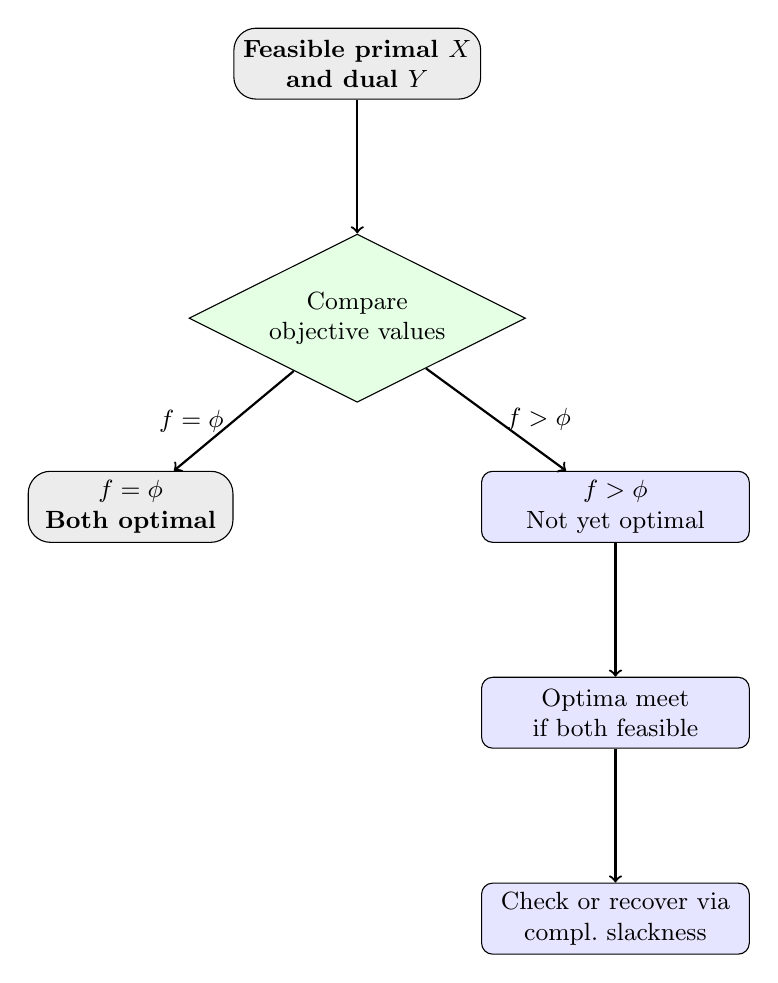
\begin{tikzpicture}[node distance=1.7cm]
\node (A) [term] {Feasible primal $X$\\and dual $Y$};
\node (B) [dec, below=of A] {Compare\\objective values};
\node (C) [term, below left=1.4cm and 0.5cm of B] {$f = \phi$\\Both optimal};
\node (D) [proc, below right=1.4cm and 0.5cm of B] {$f > \phi$\\Not yet optimal};
\node (E) [proc, below=of D] {Optima meet\\if both feasible};
\node (F) [proc, below=of E] {Check or recover via\\compl.\ slackness};
\draw [arr] (A) -- (B);
\draw [arr] (B) -- node [left, font=\small] {$f=\phi$} (C);
\draw [arr] (B) -- node [right, font=\small] {$f>\phi$} (D);
\draw [arr] (D) -- (E);
\draw [arr] (E) -- (F);
\end{tikzpicture}
\end{document}
